\documentclass[12pt]{article}
\usepackage[margin=1.3in]{geometry}
\usepackage{titlesec}
\usepackage{tikz}
\usepackage{tikz-qtree}
\usepackage{bm}

\title{Trabalho V}
\author{Bruno Samuel A. Gonçalves}
\date{}

\titleformat{\section}
  {\normalfont\Large\bfseries}{}{0em}{}

\begin{document}

\maketitle
\thispagestyle{empty}

\section{Questão 7}

\noindent Fórmula:

\[
    \neg \exists x. ((\neg Q(x) \lor Q(x)) \land (Q(x) \to \neg Q(x)))
\]

\noindent 1. Árvore de Sintaxe:

\begin{center}
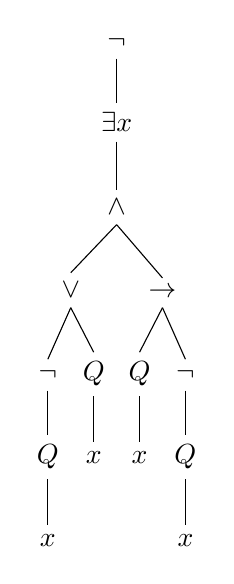
\begin{tikzpicture}
\Tree 
[.$\neg$
    [.$\exists x$
        [.$\land$
            [.$\lor$
                [.$\neg$
                    [.$Q$
                        $x$
                    ]
                ]
                [.$Q$
                    $x$
                ]
            ]
            [.$\to$
                [.$Q$
                    $x$
                ]
                [.$\neg$
                    [.$Q$
                        $x$
                    ]
                ]
            ]
        ]
    ]
]
\end{tikzpicture}
\end{center}

\noindent 2. Classificação:

\begin{center}
    \textbf{Falsa} \\
    $(Q(x) \to \neg Q(x)) \to \bm{\bot}$
\end{center}

\end{document}
